\documentclass[mm,10pt,a4paper]{simple_style}  
%%\usepackage{lastpage}
%%%
%%\usepackage{fancyhdr}
%%\fancyfoot[C]{Page \thepage\ of \pageref{LastPage}}


\usepackage[pscoord]{eso-pic}
\usepackage{qrcode}
\newcommand{\myqr}{\qrcode{https://prateekrajgautam.github.io/}}
\usepackage{graphicx}
\newcommand\BackgroundPic{%
%    \put(-10,-65){%
	\put(122,-10){
	        \parbox[b][\paperheight]{\paperwidth}{%
            %           \vfill
            \centering
%	\includegraphics[width=2cm]{./photo.jpg}
	      \myqr
	\vspace{1em}
            \vfill
}}}
\newcommand\ProfilePic{%
%    \put(-10,-65){%
	\put(-320,-10){
	        \parbox[b][\paperheight]{\paperwidth}{%
            %           \vfill
            \centering
	\includegraphics[width=2cm]{./includes/photo}
	\vspace{1em}
            \vfill
}}}



\AddToShipoutPictureBG*{%
\ProfilePic
\BackgroundPic
}
\usepackage[
   backend=biber,
    style=ieee,
    url=false,
    doi=true,
    isbn=false,
    eprint=false,
	dashed=false,
	maxbibnames=5, 
	maxcitenames=4, 
	mincitenames=4,
	autolang=hyphen
  ]{biblatex}
  
%\addbibresource{journals.bib}
%\addbibresource{conferences.bib}
\addbibresource{./includes/_publications.bib}

%ISSN link
\newcommand{\issn}[1]{{\small{issn \href{https://portal.issn.org/resource/ISSN/\usebibentry{#1}{issn}}{\usebibentry{#1}{issn}}}}}

%WOS link from MJL
\newcommand{\wos}[1]{\hfill\textbf{\href{https://mjl.clarivate.com:/home?issn=\usebibentry{#1}{issn}}{\usebibentry{#1}{index}}}}

%Scopus link 
\newcommand{\scopus}[1]{\hfill\textbf{\href{https://www.scopus.com/sources.uri?issn=\usebibentry{#1}{issn}}{\usebibentry{#1}{index}}}}

\newcommand{\scopusc}[1]{\hfill\textbf{\href{\usebibentry{#1}{proof}}{\usebibentry{#1}{index}}}}

 \newcommand{\citet}[1]{\textcite{#1}}
\newcommand{\citep}[1]{\parencite{#1}}

\newcommand{\bibentry}[1]{\fullcite{#1} {\small{isbn: \usebibentry{#1}{isbn}}} \issn{#1}\scopus{#1}
}
\newcommand{\sbibentry}[1]{\fullcite{#1} {\small{isbn: \usebibentry{#1}{isbn}}} \issn{#1}\scopusc{#1}
}


\newcommand{\pubEntry}[1]{\fullcite{#1} \issn{#1} \textbf{Impact Factor:} \cusemph{\usebibentry{#1}{if}}\hfill\textbf{\wos{#1}}
}

\newcommand{\epubEntry}[1]{\fullcite{#1} \issn{#1} \hfill\textbf{\wos{#1}}
}

\newcommand{\spubEntry}[1]{\fullcite{#1} \issn{#1} \scopus{#1}
}


\newcommand{\MyLinks}{\noindent
\textbf{ORCID:\href{http://orcid.org/0000-0002-2889-4275}{0000-0002-2889-4275}, \hfill
PUBLONS:\href{https://publons.com/researcher/I-9311-2017}{I-9311-2017}, \hfill
IEEE:\href{https://ieeexplore.ieee.org/author/37086581106}{91250146}, \hfill
SCHOLAR:\href{https://scholar.google.co.in/citations?user=slZHj6cAAAAJ}{slZHj6cAAAAJ}\ }}

\long\def\referenceFileName {./includes/_publications}

\RequirePackage{usebib}
\newbibfield{doi}
\newbibfield{if}
\newbibfield{index}
\newbibfield{issn}
\newbibfield{isbn}
\newbibfield{proof}
\bibinput{./includes/_publications}




% Default font is the helvetica postscript font
\usepackage{helvet,enumitem}
\usepackage{hyperref}
\usepackage{url}
\usepackage{xcolor}
\hypersetup {
    colorlinks=true,
    linkcolor=colorlink,
    filecolor=magenta,      
    urlcolor=colorlink,
}
\usepackage[left=0.7in, right=2in, top=0.9in]{geometry}
%
% Increase text height
\textheight=700pt
%
%
%
%-------------------------------------------------------------------------------
%	NAME AND ADDRESS SECTION
%-------------------------------------------------------------------------------
\name{Dr. Prateek Raj Gautam}
\qualification{\normalsize{\textbf{Ph.D.}, Electronics and Communication Engineering,\\ \textbf{Motilal Nehru National Institute of Technology Allahabad}}}
\emailone{dr.prateekrajgautam@gmail.com}
\emailtwo{prateek@mgeek.in}
\phone{\href{https://t.me/prateekrajgautam}{+91 - 9151404899}}
\address{E\ 540/9 Avas Vikas -- 1\\ Kalyanpur, Kanpur U.P. (208017) India}
%%\emailtwo{rel1601@mnnit.ac.in}
\website{https://prateekrajgautam.github.io}{\url{https://prateekrajgautam.github.io}}
\github{https://github.com/prateekrajgautam}{\url{https://github.com/prateekrajgautam}}
%-------------------------------------------------------------------------------
\begin{document}
\begin{resume}
%\vspace{-1em}
\fullline
\small{\hspace*{-10.2em}\MyLinks} \\
\vspace{-1em}
\sectionline
%-------------------------------------------------------------------------------
%Work Experience
%..............................................................................
\vspace{-2.5em}\section{Work Experience}
\cusemph{Assistant Professor} \timeline{August 2022 -- \textbf{Present}} \\
CSED, {\sl Centre for Advanced Studies, AKTU, Lucknow, UP}.\\
\cusemph{Assistant Professor} \timeline{July 2013 -- June 2016}\\
ECED, {\sl Allehnouse Institute of Technology, Kanpur, UP}.\\
\cusemph{Assistant Professor} \timeline{January 2012 -- July 2013} \\
ECED, {\sl Naraina College of Engineering and Technology, Kanpur, UP}.\\
\vspace{-1em}
\sectionline

%-------------------------------------------------------------------------------
%	EDUCATION SECTION
%-------------------------------------------------------------------------------
\vspace{-2em}{\section{Education}
{\cusemph{Ph. D.}} \timeline{2016--2021}\\
Electronic \& Communication Engineering {\sl (Wireless Sensor Networks)}, \textbf{\textit{Motilal Nehru National Institute of Technology Allahabad, Prayagraj (UP), India}}%, with CPI of 7.25
. Thesis Title: ``\emph{Energy Efficient 2D and 3D Localization in Wireless Sensor Networks using Single Anchor Node}''.\\

\vspace{-2em}
{\cusemph{M. Tech.}}\timeline{2009--2011}\\
Electronic \& Communication Engineering, \textbf{\textit{Harcourt Butler Technological Institute (HBTI) Kanpur (UP), India}}, with an aggregate of 67.55\%. Thesis Title: ``\emph{Generalized One Dimentional Optical Orthogonal Coding Scheme for CDMA Systems with its Grouping and Performance Analysis}''.\\ 

\vspace{-2em}
{\cusemph{B. Tech.}}\timeline{2004--2008}\\
Electronics \& Communication Engineering, \textbf{\textit{University Institute of Engineering and Technology (UIET), CSJMU Kanpur (UP), India}}, with an aggregate of 62.00\%. \\

\vspace{-2em}
{\cusemph{12 (AISSCE)}}\timeline{2004}\\
Mathematics, Biology, Physics, Chemistry, and English; \textbf{\textit{Kendriya Vidyalaya, IIT Kanpur (CB\-SE)}}, with an aggregate of 58.40\%. \\

\vspace{-2em}
{\cusemph{10 (AISSE)}}\timeline{2002}\\
Mathematics, Science, Social Studies, Hindi, and English; \textbf{\textit{Kendriya Vidyalaya, IIT Kanpur (CB\-SE)}}, with an aggregate of 67.40\%. \\
\vspace{-1em}
\sectionline
}
%%-------------------------------------------------------------------------------
%	EDUCATION SECTION
%-------------------------------------------------------------------------------
\vspace{-2em}{\section{Education}
{\cusemph{Ph. D.}} \timeline{2016--2021}\\
Electronic \& Communication Engineering {\sl (Wireless Sensor Networks)}, \textbf{\textit{Motilal Nehru National Institute of Technology Allahabad, Prayagraj (UP), India}}%, with CPI of 7.25
. Thesis Title: ``\emph{Energy Efficient 2D and 3D Localization in Wireless Sensor Networks using Single Anchor Node}''.\\

\vspace{-2em}
{\cusemph{M. Tech.}}\timeline{2009--2011}\\
Electronic \& Communication Engineering, \textbf{\textit{Harcourt Butler Technological Institute (HBTI) Kanpur (UP), India}}, with an aggregate of 67.55\%. Thesis Title: ``\emph{Generalized One Dimentional Optical Orthogonal Coding Scheme for CDMA Systems with its Grouping and Performance Analysis}''.\\ 

\vspace{-2em}
{\cusemph{B. Tech.}}\timeline{2004--2008}\\
Electronics \& Communication Engineering, \textbf{\textit{University Institute of Engineering and Technology (UIET), CSJMU Kanpur (UP), India}}, with an aggregate of 62.00\%. \\
\sectionline
}
%-------------------------------------------------------------------------------
%-------------------------------------------------------------------------------
%	RESEARCH SECTION
%-------------------------------------------------------------------------------
\vspace{-2.5em}
{\section{Research\\Interests}
Wireless Sensor Networks (\cusemph{WSNs}) / Internet of Things (\cusemph{IoTs}), Energy efficient WSN Localization, Wireless Communication, \cusemph{CDMA}, \cusemph{IDMA}, Brain Wave Mapping. Machine Learning \cusemph{AI/ML} \& Computer Vision\\
\vspace{-1em}
\sectionline
}

%-------------------------------------------------------------------------------
%-------------------------------------------------------------------------------
%	COMPUTER SKILLS SECTION
%-------------------------------------------------------------------------------
\vspace{-2.5em}
\section{Computer Skills}
{\scriptsize$\bullet$} \cusemph{MATLAB} (previous collaborations: \href{https://github.com/mgeekmatlab}{github.com/mgeekmatlab}), {\scriptsize$\bullet$} \cusemph{LabVIEW}, {\scriptsize$\bullet$} \cusemph{LTspice}, {\scriptsize$\bullet$} \cusemph{Embedded/IoT} design and programming \cusemph{Arduino IDE/PlatformIO}, {\scriptsize$\bullet$} \cusemph{CST Studio}, {\scriptsize$\bullet$} \cusemph{KiCAD},\\ 
{\scriptsize$\bullet$} \cusemph{LaTeX} (pgfplots/tikz/beamer), {\scriptsize$\bullet$} \cusemph{Gnuplot}, {\scriptsize$\bullet$} \cusemph{Word/Excel, LibreOffice},\\
{\scriptsize$\bullet$} Photoshop/Corel Draw/Inkscape/GIMP, {\scriptsize$\bullet$} \cusemph{Blender}, \\
{\scriptsize$\bullet$} \cusemph{Github}, {\scriptsize$\bullet$} \cusemph{Web design}: \cusemph{HTML}, \cusemph{CSS}, \cusemph{Javascript}, Github pages, Jekyll, hosting and server management, \cusemph{WordPress}, \cusemph{Django} \emph{(Designed and hosted conference (vcas2018) website at MNNIT ECED, online at \href{http://mnnit.ac.in/vcas2018}{mnnit.ac.in/vcas2018})}, \\
{\scriptsize$\bullet$} \cusemph{Python} (tkinter/kivy/eel) \emph{(Designed GUI based hotspot software online at \href{https://fwh.mgeek.in}{fwh.mgeek.in})}, \emph{(Form filler software online at \href{https://formhelper.mgeek.in}{formhelper.mgeek.in})}. {\scriptsize$\bullet$} Designed \cusemph{GeneratorJS} library in JavaScript and \cusemph{PyGenerator} module in python for website templating and front-end design available online at \href{https://generatorjs.mgeek.in}{generatorjs.mgeek.in}. {\scriptsize$\bullet$} \cusemph{Docker}, \cusemph{Proxmox}. {\scriptsize$\bullet$} \cusemph{Linux}, bash, Windows, and \cusemph{NixOS}.\\
%,{\scriptsize$\bullet$}Good typing speed, {\scriptsize$\bullet$} Adaptability, 
\vspace{-1em}
\sectionline
%-------------------------------------------------------------------------------
%-------------------------------------------------------------------------------
%      PUBLICATIONS 
%-------------------------------------------------------------------------------
\vspace{-2.5em}
\section{Publications\\ Journal$(J)$\\Conference$(C)$}
%\subsection{Journals}
\vspace{-1em}
%\hspace*{-10.2em}
\small{
  \begin{enumerate}[label={\textbf{[$J$\arabic*]}\ }]
\item \pubEntry{J1}
\item \pubEntry{J2}
\item \pubEntry{J3}
\item \pubEntry{J4}
\item \pubEntry{J5}
\item \pubEntry{J6}
\item \pubEntry{J7}
\item \pubEntry{J8}
\item \pubEntry{J9}
\item \pubEntry{J10}
\item \pubEntry{J11}
\item \pubEntry{J12}
\item \pubEntry{J13}
\item \pubEntry{J14}
\item \spubEntry{S1}
\item \spubEntry{S2}
\item \spubEntry{S3}
\item \spubEntry{S4}
%\item \spubEntry{S5}
\end{enumerate}
\vspace{-1em}
%\subsection{Conferences}
\begin{enumerate}[label={\textbf{[$C$\arabic*]}\ }]
\item \sbibentry{C1}
\item \bibentry{C2}
\item \bibentry{C3}
\item \bibentry{C4}
\item \sbibentry{C5}
\item \sbibentry{C6}
\item \bibentry{C7}
\item \bibentry{C8}
\item \bibentry{C9}
\end{enumerate}
}

\vspace{-3em}
\sectionline
%-------------------------------------------------------------------------------
%-------------------------------------------------------------------------------
%       Paper Presented
%-------------------------------------------------------------------------------
\vspace{-2.5em}
\section{Paper presented}
``\cusemph{{Localization of Sensor Nodes in WSNs using Three Dimensional Angle of Arrival detection at BS}}" In {\sl 1st International Conference on VLSI, Communication and Signal Processing (VCAS 2018)} at MNNIT Allahabad (UP) India. \timeline{29th November to 1st December 2018}\\

\vspace{-1.5em}
``\cusemph{Sensor Localization in {WSNs} Using Rotating Directional {-} Antenna at the Base Station.}" In {\sl 2nd International Conference on VLSI, Communication and Signal Processing (VCAS 2019)} at MNNIT Allahabad (UP) India. \timeline{21st -- 23rd October 2019}\\
\vspace{-1em}
\sectionline

%-------------------------------------------------------------------------------
%-------------------------------------------------------------------------------
%	PEER REVIEWER
%-------------------------------------------------------------------------------
\vspace{-2.5em}
\section{Journal Reviewer and Editor}
$\bullet$ IEEE Transactions on Industrial Informatics WOS (3), $\bullet$ IET Communications WOS (6),\\ $\bullet$ International Journal of Distributed Sensor Networks WOS (1), $\bullet$ Asian Journal of Cardiology Research (1), $\bullet$ SN Applied Sciences WOS (1), $\bullet$ Telecommunication Systems (3), $\bullet$ Journal of Optical Communications  (1), $\bullet$ Optica Applicata  (1), $\bullet$ International Journal of Procurement Management (1), and $\bullet$ \bf{AE} IJSAEM (8).\\
\vspace{-1em}
\sectionline

%-------------------------------------------------------------------------------
%-------------------------------------------------------------------------------
%	WORKSHOPS
%-------------------------------------------------------------------------------
\vspace{-2.5em}
\section{Workshops\\{/}FDP}
\vspace{-1em}
\begin{enumerate}[label={\textbf{\arabic*}.\ }]
%%\item One-week workshop on ``\cusemph{Antenna Design and Signal Processing for 5G Network and IoT (ADSPNIT-2017)}” held at {\sl MNNIT Allahabad}. \\-- Participated and volunteered. \timeline{27th February -4th March, 2017}
%%\item One-week workshop on ``\cusemph{Workshop on Network Simulation (WNS-2017)}” held at {\sl MNNIT Allahabad}.\\ -- Participated \timeline{8th -- 12th July, 2017}
%%\item Summer training program on ``\cusemph{VLSI Design \& 
%%Embedded System (VDES-2017)}” held at {\sl MNNIT Allahabad}. \\-- Instructed and volunteered.  \timeline{14th June -- 15th July, 2017}
%%\item One-week workshop on ``\cusemph{Communication and Antenna Design for IoT (CADIT -- 2017)}” held at {\sl MNNIT Allahabad}. \\ -- Participated and volunteered. \timeline{22nd – 27th September 2017}
\item One-week GIAN workshop ``\cusemph{Advances in Nanotechnology and its Application in Future Electronics (ANFE-2017)}” held at {\sl MNNIT Allahabad}.\\ -- Participated and volunteered \timeline{6th -- 10th November, 2017}
\item Ten days GIAN workshop on ``\cusemph{Internet of Things in Smart Living \& Cyber-Physical-Social Systems}” held at {\sl  IIT Kanpur}.\\-- Participated and volunteered.\timeline{8th -- 17th January 2018}
\item Summer training program on ``\cusemph{VLSI Design \& Embedded System (VDES-2018)}” held at {\sl MNNIT Allahabad}.\\-- Volunteered.\timeline{13th June -- 12th July, 2018}
%%\item One-week workshop on ``\cusemph{Advanced Embedded Systems \& Microelectronics (AESM-2019)}” held at {\sl MNNIT Allahabad}.\\--Volunteered.\timeline{1st -- 5th April, 2019}
\item ATAL Academy FDP on ``\cusemph{Blockchain}” held at {\sl MNNIT Allahabad}.\\-- Participated.\timeline{16th -- 20th September 2019}
\item ATAL Academy FDP on ``\cusemph{Artificial Intelligence}” held at {\sl MNNIT Allahabad}.\\-- Participated.\timeline{10th -- 14th December 2019}
\item One-week short term course on ``\cusemph{Computational Physics}” held at {\sl MNNIT Allahabad}.\\-- Participated.\timeline{1st -- 5th March 2021}
\item One-week FDP on ``\cusemph{IPR Awareness and Patent Prosecution}” held at {\sl MNNIT Allahabad}.\\-- Participated.\timeline{13th -- 17th July 2021}
\item One-week FDP on ``\cusemph{Antenna Design and Microwave Applications}” held at {\sl HBTU Kanpur}.\\-- Participated.\timeline{23th -- 27th July 2021}
\end{enumerate}
\vspace{-2em}
\sectionline
%-------------------------------------------------------------------------------
%	WORKSHOPS facilitated
%-------------------------------------------------------------------------------
\vspace{-2.5em}\section{Workshops\\ facilitated}
Manuscript preparation in LaTeX,\\ Programming with 8051 micro-controller.
\vspace{-1em}
\\\sectionline
%-------------------------------------------------------------------------------
%	Interests
%-------------------------------------------------------------------------------
\vspace{-2.5em}
\section{Awards\\and\\Other\\Achievements}
\vspace{-.5em}
\begin{enumerate}[label={\textbf{\arabic*}.\ }]
\item Awarded national scholarship ``\textbf{RG-NFSC}'' from UGC.\timeline{2017-2021}
\item Offered national scholarship ``\textbf{MANF}''  from UGC based on \textbf{NET score} \timeline{2020}
\item Eight times \cusemph{GATE} qualified. \timeline{2008, 2009, 2012, 2013, 2014, 2016, 2017, and 2020}
\item Three times \cusemph{NET} (Electronics Science) qualified. \timeline{Jul-2016, Jan-2017, and Dec-2019}
\item Member of \cusemph{IEEE}, \cusemph{IEEE Industrial Electronics Society}, \cusemph{IEEE Microwave Theory and Techniques Society}, and \cusemph{IEEE Broadcast Technology Society}.
\item \cusemph{NPTEL Online Certification} on MATLAB for Numerical Computations.
\end{enumerate}
\vspace{-2em}
\sectionline

%-------------------------------------------------------------------------------
%-------------------------------------------------------------------------------
%	References
%-------------------------------------------------------------------------------
\vspace{-2em}
\section{References}
\vspace{-1em}
\begin{enumerate}[label={\textbf{\arabic*}.\ }]
\item \textbf{Dr. Arvind Kumar} \emph{Associate Professor}, ECED, MNNIT Allahabad, Teliyarganj, Prayagraj, UP 211004, \textbf{E.Mail: }\href{mailto:arvindk@mnnit.ac.in}{arvindk@mnnit.ac.in} \textbf{Mob:}\emph{7081869266},\hfill \emph{-- Ph.D. Thesis Supervisor}
\item \textbf{Dr. Arun Prakash} \emph{Associate Professor}, ECED, MNNIT Allahabad, Teliyarganj, Prayagraj, UP 211004, \textbf{E.Mail: }\href{mailto:arun@mnnit.ac.in}{arun@mnnit.ac.in} \textbf{Mob:}\emph{9794008282}.
\item \textbf{Dr. Basant Kumar} \emph{Associate Professor}, ECED, MNNIT Allahabad, Teliyarganj, Prayagraj, UP 211004, \textbf{E.Mail: }\href{mailto:singhbasant@mnnit.ac.in}{singhbasant@mnnit.ac.in} \textbf{Tel:}\emph{+91-0532-2271468}.
\item \textbf{Dr. Vijay Shankar Tripathi} \emph{Professor}, ECED, MNNIT Allahabad, Teliyarganj, Prayagraj, UP 211004, \textbf{E.Mail: }\href{mailto:vst@mnnit.ac.in}{vst@mnnit.ac.in} \textbf{Mob:}\emph{8004818000}.
\item \textbf{Dr. Ram Chandra Singh Chauhan} \emph{Associate Professor}, ECED, IET, Sitapur Road, Lucknow UP, \textbf{E.Mail: }\href{mailto:ram1.hbti@gmail.com}{ram1.hbti@gmail.com} \textbf{Mob:}\emph{9336050184}. \hfill\emph{-- M.Tech. Dissertation Supervisor}
\end{enumerate}
\vspace{-2.5em}
\sectionline

%-------------------------------------------------------------------------------
%-------------------------------------------------------------------------------
%	PERSONAL PROFILE
%-------------------------------------------------------------------------------
\vspace{-2em}
\section{Personal Profile}
\vspace{-2.5em}
\begin{tabbing}
\=\hspace{7em}\= \kill \\
\>Name:\>\textbf{{Dr. Prateek Raj Gautam}} \\
\>DOB: \>\textbf{{17 June 1987}}\\ 
\>Email: \>\textbf{{\href{mailto:prateekrajgautam@gmail.com}{prateekrajgautam@gmail.com}}},  \textbf{{\href{mailto:prateek@cas.res.in}{prateek@cas.res.in}}} \\
\>Mobile: \>\textbf{{\href{https://t.me/prateekrajgautam}{+91- 9151 404 899}}}\\
\>Address: \>\textbf{{E 540\/9 Avas Vikas 1, Kalyanpur, Kanpur, UP - 208017, India}}\\
\>Father’s name: \>\textbf{{Mr. Shriram Gautam}} \\
\>Mother’s name: \>\textbf{{Mrs. Archana Gautam}}
\end{tabbing}
\vspace{-2em}
\sectionline
%-------------------------------------------------------------------------------
%-------------------------------------------------------------------------------
%	Declaration
%-------------------------------------------------------------------------------
\vspace{-2em}
\section{Declaration}
\vspace{-.5em}
{\sl I hereby declare that the above information given is true to the best of my knowledge and I bear the responsibility for the correctness of the above-mentioned particulars.}\\

\includegraphics[width=3.5cm]{./includes/sign}\\
\vspace{-6pt}
\today
\vspace{1em}\\
\sectionline

\end{resume}
\nocite{*}
%\printbibliography
\end{document}
